%% Vishal Kumar Sharma -- CV (two pages, A4)
%% Layout follows the widely used "Jake's Resume" LaTeX format, with a photo header.
%% Build:   cd cv && pdflatex Vishal_CV.tex && cp Vishal_CV.pdf ../pdfs/Vishal_CV.pdf
%% Needs only standard TeX Live packages (works on Overleaf as-is).
\documentclass[a4paper,10pt]{article}

\usepackage[T1]{fontenc}
\usepackage[utf8]{inputenc}
\usepackage[scaled=0.92]{helvet}
\renewcommand{\familydefault}{\sfdefault}
\usepackage[a4paper,left=1.5cm,right=1.5cm,top=1.2cm,bottom=1.2cm]{geometry}
\usepackage{graphicx}
\usepackage{tabularx}
\usepackage{enumitem}
\usepackage{titlesec}
\usepackage[dvipsnames]{xcolor}
\usepackage{marvosym}
\usepackage[hidelinks]{hyperref}
\usepackage{fancyhdr}

\definecolor{accent}{HTML}{0B5C8A}
\definecolor{muted}{HTML}{555555}

\pagestyle{fancy}
\fancyhf{}
\renewcommand{\headrulewidth}{0pt}
\cfoot{\color{muted}\footnotesize Vishal Kumar Sharma \textperiodcentered{} CV \textperiodcentered{} page \thepage}
\setlength{\parindent}{0pt}
\raggedright

\titleformat{\section}{\color{accent}\large\bfseries\scshape}{}{0pt}{}[\vspace{-4pt}{\color{accent}\titlerule[0.8pt]}]
\titlespacing*{\section}{0pt}{9pt}{5pt}

\setlist[itemize]{leftmargin=1.1em,itemsep=1pt,topsep=2pt,parsep=0pt,label={\color{accent}\textbullet}}

% \role{Title}{Dates}{Organisation}{Location}
\newcommand{\role}[4]{%
  \begin{tabularx}{\textwidth}{@{}X r@{}}
    \textbf{#1} & \textbf{#2}\\
    \textit{#3} & \textit{\color{muted}#4}\\
  \end{tabularx}\vspace{-3pt}}
% \pub{Year}{Text}
\newcommand{\pub}[2]{\item[\textbf{#1}] #2}

\begin{document}

%----------------------------------------------------------- HEADER
\begin{minipage}[c]{0.15\textwidth}
  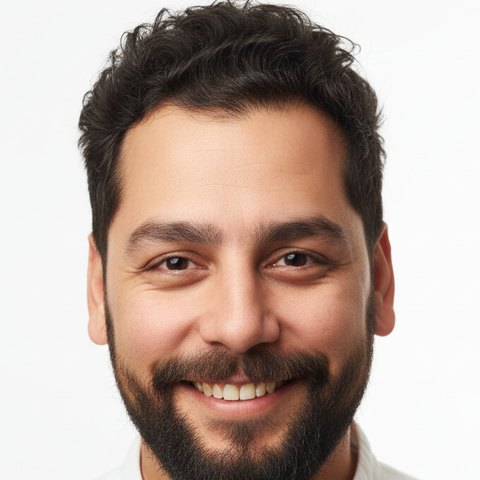
\includegraphics[width=\linewidth]{../assets/profile.jpg}
\end{minipage}\hfill
\begin{minipage}[c]{0.82\textwidth}
  {\fontsize{24}{26}\selectfont\bfseries Vishal Kumar Sharma}\\[4pt]
  {\large\color{accent} Application Manager, Legal \& General \textperiodcentered{} PhD Researcher \textperiodcentered{} Author}\\[6pt]
  \small
  \Mobilefone~+44 7519 686179 \quad
  \Letter~\href{mailto:vishalsharma3003@gmail.com}{vishalsharma3003@gmail.com} \quad
  \Mundus~Brighton, United Kingdom\\[2pt]
  \href{https://linkedin.com/in/vishalsharma3003/}{linkedin.com/in/vishalsharma3003} \quad
  \href{https://github.com/vishalsharma3003}{github.com/vishalsharma3003} \quad
  \href{https://stackoverflow.com/users/12262111/vishal-sharma}{stackoverflow.com/users/12262111}
\end{minipage}

%----------------------------------------------------------- PROFILE
\section{Profile}
Analytical data scientist and strategist with \textbf{11 years} of cross-industry experience in analytics, machine learning and predictive modelling across insurance, banking, real estate and manufacturing. Builds production analytics products and interactive R~Shiny applications that drive business decisions, backed by doctoral research in \textbf{multimodal deepfake detection} and peer-reviewed work in IEEE and Springer venues.

%----------------------------------------------------------- EXPERIENCE
\section{Experience}
\role{Application Manager}{Apr 2023 -- Present}{Legal \& General Insurance}{United Kingdom}
\begin{itemize}
  \item Lead development of risk-accumulation analytics: Shiny applications for underwriters with interactive mapping (leaflet) and visualisation (plotly, highcharts).
  \item Built a GIP claims-prediction model (binary classification in Dataiku and R) with full EDA and stakeholder reporting.
\end{itemize}

\role{Senior Analyst -- Pricing / R Shiny Developer}{Jul 2021 -- Apr 2023}{Equipped Analytical Intelligence}{}
\begin{itemize}
  \item Priced portfolios for investment opportunities of up to \textbf{\pounds150M}, including NPL and securitisation pricing with risk--return analysis.
  \item Developed predictive models for loan defaults, collections and prepayments; led dashboard-optimisation initiatives.
\end{itemize}

\role{Data Scientist}{Jan 2020 -- Jun 2021}{CBRE}{}
\begin{itemize}
  \item Built the Portfolio Transformation Calculator for COVID-19 impact analysis and the ML-powered \textit{CBRE Pathfinder} dashboard (Python--R via Flask APIs on AWS).
  \item Delivered location-intelligence systems (Google Maps API), automated EDA tools and portfolio dashboards for Fortune 500 clients.
\end{itemize}

\role{Junior Data Scientist}{Jul 2015 -- Jan 2020}{Sopra Banking Software}{}
\begin{itemize}
  \item Banking platform development for NS\&I (UK); churn and subscription-likelihood models with interactive R~Shiny campaign analysis.
  \item Developed house-price prediction and customer-segmentation models.
\end{itemize}

%----------------------------------------------------------- EDUCATION
\section{Education}
\role{Ph.D., Computer Science and Engineering}{2021 -- 2026}{Amity University, Noida}{}
\small Thesis: \textit{Detecting DeepFake Videos Based on Spatio-temporal Features \& Audio-Visual Modalities Using Artificial Intelligence}\normalsize\\[3pt]
\role{Masters in Software Systems (Data Science)}{2017 -- 2020}{BITS Pilani}{CGPA 8.47/10}\\[3pt]
\role{B.Tech., Computer Science \& Engineering}{2011 -- 2015}{Inderprastha Engineering College, Ghaziabad}{72.9\%}

%----------------------------------------------------------- SKILLS
\section{Technical Skills}
\begin{tabularx}{\textwidth}{@{}l X@{}}
  \textbf{Languages}     & R, Python, SQL, JavaScript, Java, Shell scripting\\
  \textbf{ML \& AI}      & Machine learning, deep learning, statistical modelling, NLP, computer vision, prompt engineering\\
  \textbf{Platforms}     & R Shiny, Dataiku, Snowflake, AWS, TensorFlow, Tableau, Power BI, Jupyter\\
  \textbf{Visualisation} & ggplot2, Plotly, Leaflet, Highcharts, D3.js\\
\end{tabularx}

%----------------------------------------------------------- PROJECTS
\section{Key Projects}
\begin{itemize}
  \item \textbf{Accumulation of Risk Analytics} (insurance) -- Shiny application for underwriters to calculate risk accumulation, with interactive leaflet mapping.
  \item \textbf{GIP Claims Prediction} (machine learning) -- classification model predicting claim-payment likelihood, built in Dataiku and R.
  \item \textbf{Portfolio Pricing Engine} (financial analytics) -- NPL and securitisation pricing for opportunities up to \pounds150M with risk--return analysis.
  \item \textbf{CBRE Pathfinder} (real-estate tech) -- ML-powered property-decision dashboard integrating Python and R through Flask APIs on AWS.
  \item \textbf{Banking Churn Prediction} (banking) -- end-to-end churn model for NS\&I with R~Shiny visualisations and automated campaign analysis.
\end{itemize}

%----------------------------------------------------------- BOOK
\newpage
\section{Book}
\textbf{Prompt Engineering for Production Systems: Building Reliable, Testable, and Maintainable LLM Applications} (First Edition, 2026).
A practitioner's guide to evaluation, regression testing, reliability, observability and security for LLM applications.
\href{https://www.amazon.co.uk/dp/B0HHY145SD}{\color{accent}Available on Amazon}.

%----------------------------------------------------------- PUBLICATIONS
\section{Selected Publications}
\begin{itemize}[leftmargin=2.7em,labelwidth=2.2em,align=left,itemsep=3pt]
  \pub{2026}{\textbf{Point-based Spatio-temporal Convolution and Dual-channel Attention for Lightweight Multimodal Deepfake Detection.} V.\,K.~Sharma, S.~Rawat, Q.~Caudron. \textit{Iranian Journal of Science and Technology, Trans.\ Electrical Engineering}, Springer. \href{https://doi.org/10.1007/s40998-026-01247-4}{doi:10.1007/s40998-026-01247-4}}
  \pub{2026}{\textbf{Audio-Visual Fusion for Deepfake Video Detection: A Deep Learning Framework.} V.\,K.~Sharma, R.~Garg, Q.~Caudron. ICAAAIML 2023, \textit{Lecture Notes in Electrical Engineering} vol.~1464, Springer, pp.~119--133. \href{https://doi.org/10.1007/978-981-95-0148-9_10}{doi:10.1007/978-981-95-0148-9\_10}}
  \pub{2025}{\textbf{Enhancing Deepfake Detection Through Dynamics of Facial Expressions.} V.\,K.~Sharma, S.~Rawat. \textit{6th Int.\ Conf.\ on Intelligent Communication Technologies and Virtual Mobile Networks (ICICV)}, IEEE. \href{https://doi.org/10.1109/ICICV64824.2025.11085942}{doi:10.1109/ICICV64824.2025.11085942}}
  \pub{2024}{\textbf{A Systematic Literature Review on Deepfake Detection Techniques.} V.\,K.~Sharma, R.~Garg, Q.~Caudron. \textit{Multimedia Tools and Applications}, Springer. \href{https://doi.org/10.1007/s11042-024-19906-1}{doi:10.1007/s11042-024-19906-1}}
  \pub{2024}{\textbf{Stronger Together: Crafting Successful Industry--Academia Partnerships.} Springer book chapter. \href{https://doi.org/10.1007/978-981-96-0201-8_51}{doi:10.1007/978-981-96-0201-8\_51}}
  \pub{2024}{\textbf{Spatio-Temporal Convolutional Neural Networks for Deepfake Detection: An Empirical Study.} V.\,K.~Sharma, R.~Garg, Q.~Caudron. \textit{2nd Int.\ Conf.\ on Informatics (ICI)}, IEEE. \href{https://doi.org/10.1109/ICI60088.2023.10420892}{doi:10.1109/ICI60088.2023.10420892}}
\end{itemize}

%----------------------------------------------------------- RECOGNITION
\section{Recognition}
\begin{itemize}
  \item \textbf{Best Shiny App Award} -- first prize for the best Shiny application within the organisation.
  \item \textbf{Customer Delight Award} -- for consistency and commitment to quality deliveries.
\end{itemize}

\end{document}
